\chapter{Método Proposto}\label{meto}

Para concluir com êxito o desenvolvimento deste trabalho e consequentemente os objetivos propostos, o método utilizado para solução do problema é composto das seguintes etapas sequenciais:

Como já foi dito o banco de redações UOL foi desenvolvido e armazenado em páginas HTML, o que permite o uso de um \textit{Web Crawler}, um algoritmo que explora a estrutura de grafo da \textit{Web} para navegar de uma página para outra. A Figura ~\ref{fig:metodologia_1} ilustra a etapa que o\textit{Web Crawler} recupera as páginas, filtra as redações avaliadas e coleta cada uma para um repositório local.

\begin{figure}[H]
\begin{center}
    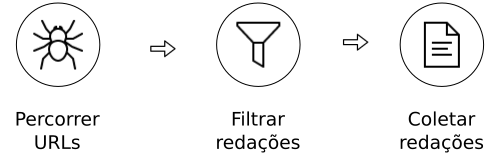
\includegraphics[scale=0.75]{figuras/metodologia_1.png}
\end{center}
\caption{Um \textit{Web Crawler}, navega entre as páginas HTML do banco de redações UOL de forma metódica e automatizada indexando textos de redações que posteriomente serão filtrados e coletados.}
\label{fig:metodologia_1}
\end{figure}

Na etapa subsequente a Figura ~\ref{fig:metodologia_2} ilustra a normalização dos textos, que consiste em uma técnica de remoção de caracteres não alfa-numéricos presentes no HTML e espaços desnecessários, tal que o valor textual ainda seja o mesmo que o original. Após a normalização será organizado as as diversas partes que compõem a redação (tema, título, texto e nota) em uma estrutura JSON para armazenamento e uso futuro. 

\begin{figure}[H]
\begin{center}
    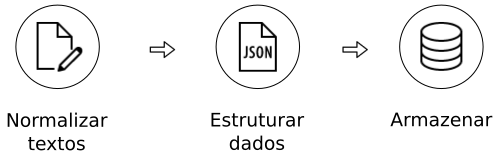
\includegraphics[scale=0.75]{figuras/metodologia_2.png}
\end{center}
\caption{Os textos são submetidos aos algoritmos de normalização e posteriormente estruturados e armazenados no padrão JSON.}
\label{fig:metodologia_2}
\end{figure}

Na terceira etapa ilustrada pela Figura ~\ref{fig:metodologia_3} será utilizada a ferramenta de mineração de dados \textit{Orange} ~\cite{JMLR:demsar13a}. Será necessário realizar estudo e análise para obter o conhecimeto necessário para desenvolvimento de um fluxo de trabalho, seleção e treinamento dos modelos classificadores, concluindo todos os objetivos propostos nesta etapa.

\begin{figure}[H]
\begin{center}
    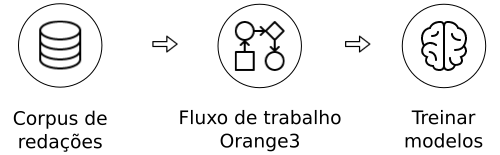
\includegraphics[scale=0.75]{figuras/metodologia_3.png}
\end{center}
\caption{O \textit{corpus} será utilizado em um fluxo de trabalho da ferramenta \textit{Orange} para treinar os modelos classificadores.}
\label{fig:metodologia_3}
\end{figure}

A quarta e última etapa é ilustrada pela Figura ~\ref{fig:metodologia_4}, onde os modelos classificadores previamente ajustados e treinados serão submetidos aos testes de Acurácia (taxa de predições corretas ou incorretas realizada pelo modelo para um determinado conjunto de dados), \textit{Overfitting} (super-ajustamento que ocorre quando o modelo se especializa nos dados utilizados no seu treinamento) e \textit{Noise} (\textit{noise} ou ruido é classificação errada do conjunto de dados de entrada), os resultados serão representados e comparados graficamente.
\begin{figure}[H]
\begin{center}
    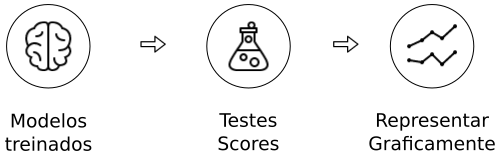
\includegraphics[scale=0.75]{figuras/metodologia_4.png}
\end{center}
\caption{O modelos ajustados e treinados serão submetidos a testes, e os resultados comparados graficamente.}
\label{fig:metodologia_4}
\end{figure}
